%! Author = danielmendes
%! Date = 05.01.25
\chapter{Grundlagen}\label{ch:grundlagen}

In diesem Kapitel werden die Grundlagen der Bachelorarbeit betrachtet, die in den späteren Kapiteln für die Durchführung der Benchmark-Tests und Analysen erforderlich sind.
Zunächst werden die einzelnen Schritte dargelegt, um die im vorherigen Kapitel~\ref{sec:auswahl-der-tools} ausgewählten Tools korrekt zu verwenden.
Besonders beim Benchmark-Tool werden die verschiedenen Argumente untersucht, die übergeben werden können und es wird anhand eines kurzen Beispiels gezeigt, wie die Resultate dieses Tools aussehen könnten.
Danach wird eine komplexere Demonstration betrachtet, die bei späteren Tests wiederverwendet werden kann.
Zu guter Letzt wird gezeigt, wie GitHub Actions funktionieren, bei den Benchmark-Tests Aufwand ersparen und wie die Workflows sowohl zeitlich als auch ressourcenschonend optimiert werden können.

\section{Überblick über die Tools}\label{sec:einfuhrung-in-die-tools}

Um die Tools näher zu erläutern, ist die Grundvoraussetzung zuallererst ein laufendes Datenbankmanagementsystem, in diesem Fall MySQL\@.
Dabei ist es egal, ob es lokal auf einem Rechner oder über Docker in einem GitHub CI/CD-Workflow gestartet wird.
Wichtig ist aber, dass man sich die Zugangsdaten, bestehend aus Benutzer- und Passwortdaten, abspeichert, da diese gebraucht werden, um den Benchmark-Test mit Sysbench zu starten.
Nachdem das RDBMS gestartet worden ist, muss zunächst eine Datenbank erstellt werden:

\vspace{-4pt}
\lstinputlisting[
    language=sql,
    label={lst:tools-create-db},
    style=custom_daniel,
]{Scripts/Tools/01_database.sql}
\vspace{-8pt}

Neben der erfolgreichen Erstellung der Datenbank muss ebenfalls das Tool Sysbench installiert werden.
Auf einem Linux-basierten System kann dies wie folgt umgesetzt werden:

\vspace{-4pt}
\begin{lstlisting}[language=bash]
sudo apt install sysbench
\end{lstlisting}
\vspace{-8pt}

Damit die Grafiken erstellt werden können, werden zusätzlich die Tools \texttt{Gnuplot} und \texttt{Pandas} in Kombination mit \texttt{matplotlib} benötigt.
Die Befehle \texttt{sudo apt} und \texttt{pip} müssen je nach Betriebssystem beispielsweise durch \texttt{brew} und \texttt{pip3} ersetzt werden.

\vspace{-4pt}
\begin{lstlisting}[language=bash]
sudo apt install gnuplot
pip install pandas matplotlib
\end{lstlisting}
\vspace{-9pt}

Damit wurden alle Abhängigkeiten eingerichtet und im nächsten Schritt muss man sich mit den Tools vertraut machen.
Der Hauptfokus wird dabei auf Sysbench gerichtet.
Um mit Sysbench zu interagieren, verwendet man Shell-Befehle, bei denen verschiedene Parameter angegeben werden können, um spezifische Tests durchzuführen.
Die folgende Übersicht zeigt die Argumente, die übergeben werden müssen, sowie solche, die optional angegeben werden können:

\vspace{-5pt}
\begin{itemize}
    \setlength{\itemsep}{-7pt}
    \item \textbf{\texttt{db-driver}}: Treiber der Datenbank, in diesem Fall \textbf{\texttt{mysql}}
    \item \textbf{\texttt{mysql-host}}: Hostname oder IP-Adresse des Servers (Standard: \texttt{localhost})
    \item \textbf{\texttt{mysql-user}}: Benutzername der Datenbank
    \item \textbf{\texttt{mysql-password}}: Passwort des DB-Benutzers (kann weggelassen werden, wenn keine Authentifizierung erforderlich ist)
    \item \textbf{\texttt{mysql-db}}: Name der zu verwendenden Datenbank, hier: \textbf{\texttt{sbtest}}
    \item \textbf{\texttt{time}}: Laufzeit des Benchmarks in Sekunden (verpflichtend)
    \item \textbf{\texttt{report-interval}}: Intervall in Sekunden, in dem Zwischenergebnisse angezeigt werden (Standard: nur Gesamtstatistiken am Ende)
    \item \textbf{\texttt{tables}}: Anzahl der zu erstellenden Tabellen (Standard: 1)
    \item \textbf{\texttt{table-size}}: Anzahl der Datensätze pro Tabelle (optional)
\end{itemize}

Einige dieser genannten Parameter, wie z.B.\ \texttt{db-driver}, dienen dazu die Verbindung mit den Datenbankmanagementsystem herzustellen.
Mit den anderen Argumenten kann man die Einzelheiten des Benchmarks genauer bestimmen.
So kann beispielweise festgelegt werden, wie lange der Benchmark laufen soll und wie häufig die Teilergebnisse geloggt werden.
Damit fehlen aber noch die Informationen über die Tabellen und die Abfragen, die getestet werden sollen.
Dies kann, wie im Abschnitt~\ref{sec:auswahl-der-tools} beschrieben, entweder über explizite Lua-Skripts oder mithilfe von vordefinierte Testtypen in Sysbench geregelt werden.
Durch die vordefinierten Typen lässt sich schnell kontrollieren, ob die Parameter zur Datenbankverbindung korrekt sind, ohne dafür SQL-Befehle oder Lua-Skripte schreiben zu müssen.
Unter anderen kann man zwischen dem reinen Einfügen von Daten (\texttt{oltp\_insert}), dem Abfragen von Daten (\texttt{oltp\_read\_only}) oder einer Kombination aus beidem (\texttt{oltp\_read\_write}) wählen.
Als letztes muss noch festgelegt werden, welche der folgenden Methoden ausgeführt werden soll:

\begin{itemize}
    \setlength{\itemsep}{-3pt}
    \item \textbf{prepare}: Bereitet die Datenbank für den Test vor, u.a.\ das Erstellen der Tabellen.
    \item \textbf{run}: Je nach Testtyp führt diese Methode die spezifizierten Operationen aus und misst dabei die Performance.
    \item \textbf{cleanup}: Stellt die Datenbank in ihren ursprünglichen Zustand zurück.
\end{itemize}

Die Methoden sowie der Testtyp oder der Pfad des Lua-Skripts werden am Ende der Sysbench-Befehlszeile hinzugefügt.
Als Beispiel wird der Testtyp \texttt{oltp\_read\_write} zusammen mit der Methode \texttt{RUN} ausgewählt.
Die Query könnte wie folgt aussehen, wobei die Werte für die Variablen \texttt{YOUR\_USER} und \texttt{YOUR\_PASSWORD} durch die tatsächlichen Benutzerdaten ersetzt werden müssen:

\vspace{-5pt}
\begin{lstlisting}[style=custom_daniel,label={lst:tools-sysbench-run}]
sysbench oltp_read_write \
  --db-driver=mysql \
  --mysql-user=YOUR_USER \
  --mysql-password=YOUR_PASSWORD \
  --mysql-db="sbtest" \
  --time=10 \
  --report-interval=1 \
  run
\end{lstlisting}
\vspace{-5pt}

Wenn man nur diese Query ausführt, fällt er auf, dass sie scheitert.
Die Fehlermeldung lautet dabei wie folgt:

\begin{lstlisting}[style=custom_daniel,label={lst:tools-error-without-prepare}]
FATAL: MySQL error: 1146 "Table 'sbtest.sbtest1' doesn't exist"
\end{lstlisting}

Der entstandene Fehler wird dadurch verursacht, dass die Tabelle \texttt{sbtest1} nicht erstellt worden ist.
Daher muss vor der Ausführung der \texttt{RUN}-Methode zunächst die \texttt{PREPARE}-Methode durchgeführt werden.
Und um die Datenbank wieder in den Ausgangszustand zu versetzen, muss nach dem \texttt{oltp\_read\_write}-Testtyp auch die \texttt{CLEANUP}-Methode aufgerufen werden.
Um sich die manuelle Ausführung dieser drei Befehle in der korrekten Reihenfolge zu sparen, bietet es sich an, ein Shell-Script zu schreiben, das diese Aufgabe übernimmt.

\vspace{-5pt}
\lstinputlisting[
    language=bash,
    caption=Ausführung der Sysbench-Methoden in korrekten Reihenfolge,
    label={lst:tools-sysbench-monitor},
    style=custom_daniel,
    basicstyle=\ttfamily\scriptsize,
]{Scripts/Tools/02_process_sysbench.sh}
\vspace{-5pt}

Beim Ausführen des Skripts gibt die \texttt{run}-Methode einmal pro Sekunde die Zwischenergebnisse in der Konsole aus, da der Wert von \texttt{report\_interval} auf 1 gesetzt ist.
Nach erfolgreichem Abschluss wird zudem eine Gesamtstatistik mit der gemessenen Kennzahlen angezeigt.
Anstatt die Ausgabe in der Konsole darzustellen, können die Werte auch in einer Log-Datei gespeichert werden.
Damit wurde bisher erläutert, wie man Sysbench verwendet, jedoch fehlt noch die Erstellung von Graphen.
Um diesen Prozess zu erleichtern, empfiehlt es sich, die relevanten Kennzahlen aus der Log-Datei zu extrahieren und mit passenden Spaltenüberschriften in einer CSV-Datei zu speichern.
Dies kann mit dem Shell-Kommando \texttt{grep} erfolgen:

\vspace{-5pt}
\lstinputlisting[
    language=bash,
    caption=Extraktion der Ergebnisse aus der Log-Datei in eine Tabelle,
    label={lst:tools-extraction-csv},
    style=custom_daniel,
    basicstyle=\ttfamily\scriptsize,
]{Scripts/Tools/03_extraction_csv.sh}
\vspace{-5pt}

Mit der erstellten CSV-Datei können Graphen entweder mit Gnuplot oder der Python-Bibliothek Pandas erzeugt werden.
Das Python-Skript muss die CSV-Datei als Argument erhalten und optional eine Liste spezifischer Messwerte, für die Graphen erstellt werden sollen.

\vspace{-5pt}
\lstinputlisting[
    language=bash,
    caption=Erstellung der Graphen aus der CSV-Datei,
    label={lst:tools-graph-generation},
    style=custom_daniel,
    basicstyle=\ttfamily\scriptsize,
]{Scripts/Tools/04_graph_generation.sh}
\vspace{-5pt}

\vspace{-5pt}
\begin{figure}[H]
    \centering
    \begin{subfigure}[t]{0.36\textwidth}
        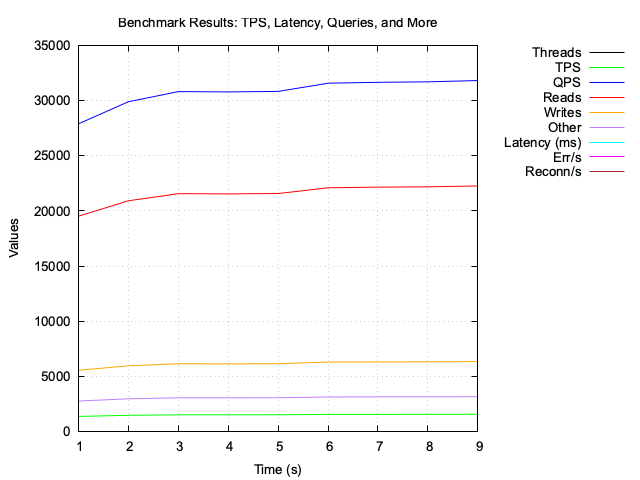
\includegraphics[width=\textwidth]{PNGs/Demo/sysbench_output}
    \end{subfigure}
    \hfill
    \begin{subfigure}[t]{0.48\textwidth}
        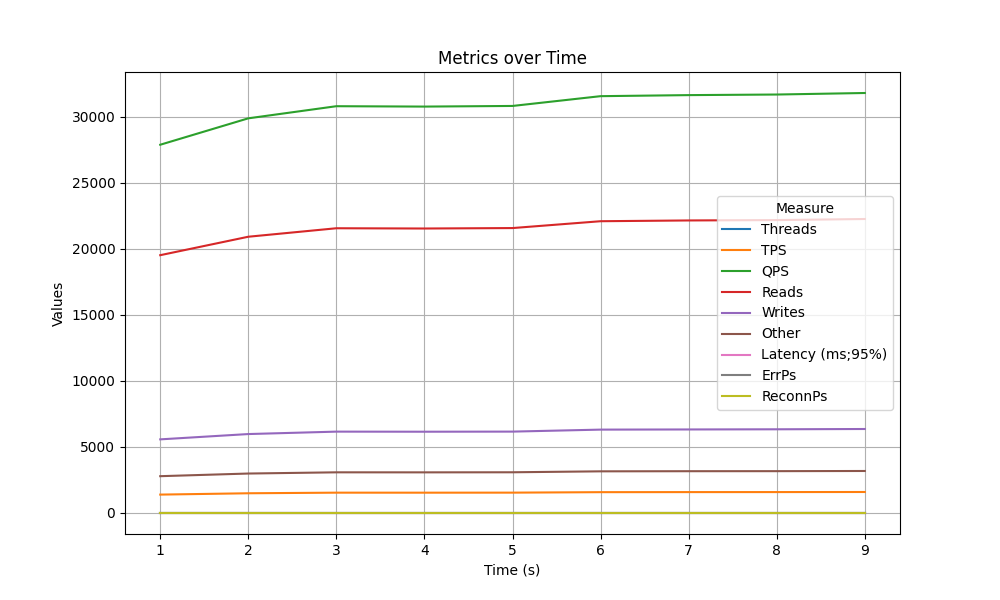
\includegraphics[width=\textwidth]{PNGs/Demo/Summary}
    \end{subfigure}
    \caption[Demo: Gnuplot vs. Pandas]{Grafik zeigt Erstellung mit Gnuplot (links) und Pandas (rechts)}
    \label{fig:demo-graph-generation}
\end{figure}
\vspace{-15pt}

Die Abbildung~\ref{fig:demo-graph-generation} zeigt die Ergebnisse der Grapherstellung.
Die dargestellten Metriken umfassen: Transaktionen, Abfragen, Fehler und Wiederverbindungen pro Sekunde (engl.\ TPS, QPS, ErrPs, ReconnPs), Anzahl der Operationen (engl.\ Reads, Writes, Other), die Latenz im 95.\ Perzentil und die Anzahl der Threads.

%Erklärung der einzelnen \textbf{Metriken}:
%\begin{itemize}
%    \setlength{\itemsep}{-5pt}
%    \item \textbf{Threads}: Anzahl der gleichzeitig verwendeten Threads $\Rightarrow$ höhere Parallelität
%    \item \textbf{TPS}: Transaktionen pro Sekunde; höherer Wert $\Rightarrow$ bessere Leistung
%    \item \textbf{QPS}: Abfragen pro Sekunde; höherer Wert $\Rightarrow$ bessere Effizienz
%    \item \textbf{Reads}: Anzahl der Leseoperationen; je mehr desto besser
%    \item \textbf{Writes}: Anzahl der Schreiboperationen; je mehr desto besser
%    \item \textbf{Other}: Andere Operationen, die weder als Reads noch Writes zählen
%    \item \textbf{Latency (ms; 95\%)}: Durchschnittliche Bearbeitungszeit (im 95.\ Perzentil); \newline niedrigere Werte $\Rightarrow$ schnellere Reaktionszeiten
%    \item \textbf{ErrPs}: Fehler pro Sekunde; niedriger Wert $\Rightarrow$ höhere Stabilität
%    \item \textbf{ReconnPs}: Wiederverbindungen pro Sekunde; häufige Wiederverbindungen $\Rightarrow$ Hinweis auf Stabilitätsprobleme
%\end{itemize}

\section{Projektaufbau}\label{sec:projektaufbau-mit-beispiel}

In dem vorausgegangenen Abschnitt wurde das Tool Sysbench und seine Funktionsweise anhand eines Demo-Projekts näher erläutert.
Damit ist die Reihenfolge und die Bedeutungen der unterschiedlichen Methoden (prepare → run → cleanup) sowie die Vorgehensweise zur Erstellung der Grafiken deutlich geworden.
Das bisherige Problem besteht jedoch darin, dass bei dem dargelegten Beispiel keine Kontrolle über die getesteten Daten besteht.
Wenn man sich die Logs genauer anschaut, dann zeigt sich, dass zwar über die Parameter des Sysbench-Befehls die Anzahl der erstellten Tabellen und eingefügten Datensätze von außen gesteuert werden kann, die genaue Implementierung jedoch auf diese Weise nicht veränderbar ist.
Genau für diese Anwendungsfälle gibt es noch die Möglichkeit ein Lua-Skript, als Parameter beim Sysbench-Aufruf mit anzugeben.
In diesen Lua-Dateien können die Implementierungen der einzelnen Methoden selbstständig gewählt werden.

Um das Vorgehen besser zu erklären, wird ein Beispiel angeschaut, bei dem zwei Tabellen erstellt und mit zufälligen Testdaten befüllt werden.
Die Abfrage, die auf Performance getestet werden soll, ist das Verbinden (Joinen) dieser beiden Tabellen.
In diesem Fall wird eine Kundentabelle mit Name, Geburtstag und Adresse sowie eine Bestelltabelle mit Artikeldetails, Bestelldatum und einem Bezug zu dem Kunden, der die Bestellung aufgibt, erstellt.
Damit nicht nur ein Beispiel dargestellt wird, ist ein Vergleich zwischen zwei verschiedenen Implementierungen erforderlich.
Der Unterschied zwischen den beiden Versionen besteht darin, dass die eine Tabelle einen Primärschlüssel vom Typ \texttt{INT} und die andere vom Typ \texttt{VARCHAR} hat.
Da Verbundoperationen aufwendig sind, wird angenommen, dass der speichereffizientere Typ \texttt{INT} Performancevorteile bietet.
Dies gilt es nun mit Benchmark-Tests genauer zu untersuchen.

Für die Durchführung der Benchmarks wird zunächst unabhängig von den Lua-Skripten mit der Spezifizierung der Tabellen begonnen, die erstellt werden sollen.
Insgesamt sind vier verschiedene \texttt{CREATE TABLE}-Befehle erforderlich, jeweils zwei pro Variante.
Sie unterscheiden sich nur im Typ des Primärschlüssels der Kundentabelle und des Fremdschlüssels in der Bestelltabelle.
Für den Fall mit \texttt{INT}, müssen die folgenden Tabellen erstellt werden:

\vspace{-10pt}
\lstinputlisting[
    language=sql,
    caption=Create Table-Befehl für Kunden,
    label={lst:tools-create-table-kunde},
    style=custom_daniel,
    basicstyle=\ttfamily\scriptsize,
]{Scripts/Grundlagen/01_Create_Table_Kunde.sql}
\vspace{-5pt}

\lstinputlisting[
    language=sql,
    caption=Create Table-Befehl für Bestellung,
    label={lst:tools-create-table-bestellung},
    style=custom_daniel,
    basicstyle=\ttfamily\scriptsize,
]{Scripts/Grundlagen/02_Create_Table_Bestellung.sql}
\vspace{-5pt}

Anschließend werden diese Befehle in der \texttt{prepare()}-Funktion verwendet.
Dafür müssen einfach die \texttt{CREATE TABLE}-Befehle an die Datenbank gesendet werden.
Wenn bestimmte Indexe oder andere Datenbankstrukturen erstellt werden sollen, müsste dies ebenfalls in der \texttt{Prepare}-Funktion erfolgen.
Dies ist ein Auszug aus der Funktion:

\vspace{-5pt}
\lstinputlisting[
    language={[5.0]Lua},
    caption=Lua-Script für die Erstellung der Tabellen,
    label={lst:tools-prepare-query},
    style=custom_daniel,
    basicstyle=\ttfamily\scriptsize,
]{Scripts/Grundlagen/03_Prepare_Query.lua}
\vspace{-5pt}

Wenn die Datenbank beispielsweise in einer Produktivumgebung läuft, dann wollen wir, dass Benchmarks möglichst wenig Einfluss auf sie haben.
Damit ist es das Ziel, dass die Datenbank möglichst nach dem Durchlauf wieder in ihrem Anfangszustand ist.
Außerdem sollte der Benchmark idempotent sein, also beliebig oft nacheinander ausgeführt werden können, ohne zu Problemen zu führen.
Wenn eine Tabelle erstellt wird, ohne sie vorher zu löschen, schlägt der \texttt{CREATE TABLE}-Befehl im nächsten Durchlauf fehl.
Dies lässt sich durch die Klausel \texttt{IF NOT EXISTS} vermeiden oder noch besser, indem die Tabelle am Ende des Benchmarks gelöscht wird.
Dafür ist die \texttt{cleanup()}-Funktion vorgesehen:

\vspace{-5pt}
\lstinputlisting[
    language={[5.0]Lua},
    caption=Lua-Script für das Aufräumen,
    label={lst:tools-cleanup-query},
    style=custom_daniel,
    basicstyle=\ttfamily\scriptsize,
]{Scripts/Grundlagen/04_CleanUp_Query.lua}
\vspace{-5pt}

Wichtig ist dabei, dass man keine Schlüsselintegritäten verletzt.
Da in diesem Fall die Tabelle \texttt{BESTELLUNG} eine Referenz auf die Tabelle \texttt{KUNDEN} hat, muss zuerst die Bestelltabelle und danach die Kundentabelle entfernt werden.

Damit wurde das Gerüst für die eigentlichen Insert- und Select-Befehle geschaffen.
Bei den Insert-Befehlen kann entweder eine Zufallszahl generiert oder aus vordefinierten Listen zufällig gewählt werden.
Allerdings muss bei den zufällig generierten Daten darauf geachtet werden, dass die Primärschlüsselbedingung nicht verletzt wird.
Deshalb bietet es sich an, mit inkrementellen Werten zu arbeiten.
In diesem Beispiel wird die \texttt{KUNDEN\_ID} fortlaufend mit dem Schleifendurchgang vergeben und die \texttt{BESTELLUNG\_ID} wird aus einer Kombination der Kundennummer und der Bestellnummer berechnet.
Es muss zudem festgelegt werden, wie viele Kunden und Bestellungen pro Kunde erstellt werden.
Um sicherzustellen, dass keine Werte in den Tabellen enthalten sind, können alle Daten aus den Tabellen entfernt werden, bevor neue hinzugefügt werden.
Damit die Performance der Insert-Query auch gemessen wird, ist es wichtig, dass die \texttt{insert()}-Funktion in der \texttt{event()}-Funktion aufgerufen wird.

%Sonst kommt es zu diesem Fehler:
%
%\begin{lstlisting}[style=custom_daniel,label={lst:tools-error_withoutevent}]
%FATAL: cannot find the event() function in Join.lua
%\end{lstlisting}
%\vspace{-5pt}

\vspace{-10pt}
\lstinputlisting[
    language={[5.0]Lua},
    caption=Lua-Script für das Einfügen von Daten,
    label={lst:tools-insert-query},
    style=custom_daniel,
    basicstyle=\ttfamily\scriptsize,
]{Scripts/Grundlagen/05_Insert_Query.lua}
\vspace{-5pt}

Die letzte Anweisung, die noch benötigt wird, ist die Select-Abfrage.
Hierbei muss man sich Gedanken machen, welche Abfrage man stellen muss, damit die untersuchten Effekte auch tatsächlich auftreten.
Da die Performance des Join-Operators untersucht wird, müssen beide Tabellen über den Fremdschlüssel verbunden werden.

\vspace{-5pt}
\lstinputlisting[
    language={[5.0]Lua},
    caption=Lua-Script für das Abfragen von Daten,
    label={lst:tools-select-query},
    style=custom_daniel,
    basicstyle=\ttfamily\scriptsize,
]{Scripts/Grundlagen/06_Select_Query.lua}
\vspace{-5pt}

Damit sind für den Vergleich mit \texttt{INT} alle vier Operationen genauer definiert, aber es fehlen noch die Veränderungen für \texttt{VARCHAR}.
Dazu muss beim \texttt{CREATE TABLE}-Befehl der Typ für die Spalten \texttt{KUNDEN\_ID} und \texttt{FK\_KUNDEN} angepasst werden und beim Einfügen muss die Variable \texttt{i} zu einem String umgewandelt werden.

Neben dem Vergleich zwischen \texttt{INT} und \texttt{VARCHAR} soll auch das Verhalten mit unterschiedlichen Längen analysiert werden.
Dadurch kann der Performanceunterschied zwischen beiden Datentypen sowie der Einfluss der Länge des Verbundoperators festgestellt werden.
Dazu wird für beide Typen eine Hilfsfunktion benötigt, die eine Zeichenkette bzw.\ eine Zahl mit einer bestimmten Länge erstellt.
Das Ergebnis der Funktion wird in der \texttt{INSERT}-Methode verwendet und zur Sicherstellung der Eindeutigkeit der \texttt{KUNDEN\_ID} mit der Schleifenvariable \texttt{i} konkateniert.
Ein Problem besteht jedoch noch darin, dass bisher nur eine Länge pro \texttt{INSERT}-Methode festgelegt werden kann.
Man könnte nun die beiden Ordner mit den Skripten duplizieren und die Längen in den neuen Dateien anpassen.
Dies würde zu extremer Redundanz führen, weshalb es eine intuitivere Lösung gibt.
Und zwar könnte man beim Aufruf des Shell-Scripts Variablen definieren, die im Skript exportiert werden und in den Lua-Dateien importiert werden können.
Die Zeile mit der festgelegten Länge könnte so aussehen:

\vspace{-5pt}
\begin{lstlisting}[language={[5.0]Lua},label={lst:tools-without-imported-length,style=custom_daniel}]
local length = 10
\end{lstlisting}
\vspace{-7pt}

Um die im Skript exportierte Variable, beispielsweise \texttt{LENGTH}, zu verwenden, muss man Folgendes tun:
\vspace{-5pt}
\begin{lstlisting}[language={[5.0]Lua},label={lst:tools-with-imported-length,style=custom_daniel}]
local length = tonumber(os.getenv("LENGTH"))
\end{lstlisting}
\vspace{-5pt}

Jetzt muss noch ermittelt werden, welche Längen überhaupt zulässig sind.
Bei \texttt{VARCHAR} gestaltet sich das einfach, da dort alle Längen bis 255 bei \texttt{VARCHAR(255)} möglich sind.
\texttt{INT} kann Werte bis \(2^{32} - 1\)~(4.294.967.295) speichern, also bis zu 10 Stellen, während \texttt{BIGINT} Werte bis \(2^{64} - 1\)~(18.446.744.073.709.551.615) kann und damit 20 Stellen umfasst.
Um größere Längen zu testen, wird der Typ der \texttt{Kundentabelle} von \texttt{INT} auf \texttt{BIGINT} geändert und es werden 4 sowie 16 Stellen als getestete Längen gewählt.

Es wurde also gezeigt, dass sich mithilfe von Lua-Skripten Tabellen gezielt erstellen, eingefügte Daten verwalten und Abfragen steuern lassen.
Um die Operationen in der korrekten Reihenfolge auszuführen und die Grafiken zu generieren, wird wieder ein Shell-Skript benötigt.
Dieses Skript soll möglichst wenige Parameter erhalten, weshalb eine festgelegte Dateistruktur erforderlich ist.
Es wird ein Ordner mit einem beliebigen Namen, z.B. \texttt{int\_queries}, benötigt, in dem sich folgende Dateien befinden:

\begin{itemize}\label{files_structure}
    \setlength{\itemsep}{-5pt}
    \item \texttt{int\_queries.lua} $\Rightarrow$ enthält die \texttt{prepare()}- und \texttt{cleanup()}-Funktionen
    \item \texttt{int\_queries\_insert.lua} $\Rightarrow$ enthält die \texttt{insert()}-Funktion
    \item \texttt{int\_queries\_select.lua} $\Rightarrow$ enthält die \texttt{select()}-Funktion
\end{itemize}

Analog muss auch ein Ordner für die Varchar-Variante erstellt werden.
Wichtig ist dabei, dass die Namen der Dateien mit dem Namen des Ordners übereinstimmen.
Das Shell-Script bedient sich dieser Struktur, führt die Lua-Skripte aus und geht die einzelnen Schritte bis zur Erstellung der Grafiken durch.
Wenn Variablen definiert werden, werden diese exportiert, um sie in den Lua-Dateien importieren zu können.
Der Dateiname dieses Orchestrators ist \texttt{sysbench\_script.sh} und man kann ihn wie folgt aufrufen:

\vspace{-10pt}
\lstinputlisting[
    language=sh,
    caption=Befehl zum Ausführen des Orchestrator Skripts,
    label={lst:tools-orchestrator-command},
    style=custom_daniel,
]{Scripts/Grundlagen/07_orchestrator_command.sh}
\vspace{-5pt}

Wenn man will, kann man mehrere Select-Abfragen ohne unterschiedliche Insert-Befehle definieren.
Dies wird später in der Bachelorarbeit nützlich sein, wenn verschiedene Indextypen untersucht und mithilfe unterschiedlicher SELECT-Abfragen überprüft wird, ob ein bestimmter Indextyp bei Abfragen verwendet wird.
Die eigentlichen Tabellen und deren Datensätze müssen dabei nicht immer wieder neu befüllt werden.
Wenn auf die Ordnerstruktur mit dem Int-Query-Beispiel zurückgekommen wird, könnte anstelle von \texttt{int\_queries\_select.lua} auch ein Ordner mit dem Namen \texttt{int\_queries\_select} erstellt werden.
In diesem Ordner können sich beliebig viele unterschiedliche Lua-Skripts befinden, die Select-Befehle durchführen.
Dadurch werden alle Select-Befehle auf der gleichen Datenbasis verglichen und es kann im Kapitel~\ref{sec:indexing-grundlagen} erkannt werden, wann der Index verwendet wird und wann nicht.

Erklärung aller möglichen Parameter des Orchestrator-Skripts:
\begin{itemize}
    \setlength{\itemsep}{-5pt}
    \item \texttt{-out}: Gibt den Pfad des Speicherorts für den Output-Ordner an
    \item \texttt{-var}: Gibt die Variablen und deren Werte im \texttt{JSON}-Format an
    \item \texttt{-scripts}: Gibt die Pfade der Ordner mit den jeweiligen Lua-Skripten im \texttt{JSON}-Format an.
    Der Schlüssel für jedes Skript ist der Pfad zur Datei.
    \vspace{2pt}
    \newline Innerhalb von \texttt{-scripts} kann man folgendes angeben:
    \begin{itemize}
        \setlength{\itemsep}{-5pt}
        \item \texttt{-vars}: Wählt aus, welche unter der \texttt{-var} angegebenen Variablen für das jeweilige Skript verwendet werden sollen
        \item \texttt{-selects}: Legt fest, welche Select-Abfragen verwendet werden sollen, wenn man mehrere in einem Ordner definiert
        \item \texttt{-db}: Gibt den Namen aller verwendeten Datenbankverbindungen aus der \texttt{db.env}-Datei in einer Liste an.
        Standardmäßig wird \texttt{MySQL} verwendet.
    \end{itemize}
\end{itemize}

Im Grundlegenden arbeitet das Orchestrator-Skripts \texttt{sysbench\_script.sh} ähnlich wie schon das Skript im Demo-Beispiel, aber durch die zusätzlichen Anwendungsfälle kommt es zu mehr Komplexität.
Zu Beginn des Skripts werden die Argumente des Skripts (siehe~\ref{lst:tools-orchestrator-command}) definiert und überprüft.
Beispielsweise wird sichergegangen, dass die für die Skripts verwendeten Parameter, in diesem Beispiel \texttt{length}, tatsächlich definiert werden mit \texttt{-var}.
Danach wird der Output-Ordner erstellt und die Spaltenüberschriften in die CSV-Dateien geschrieben.
Anschließend beginnt erst das eigentliche Durchgehen der unterschiedlichen Skripte, die unter dem Argument \texttt{-script} angegeben wurden.
Zu Beginn der Schleife entnimmt man die verwendeten Datenbanken (unter dem Argument \texttt{-db}) und die Select-Abfragen (unter dem Argument \texttt{-selects}) des aktuellen Skripts.
Daraufhin geht man in eine weitere Schleife, um die unterschiedlichen Datenbankverbindungen durchzugehen.
Innerhalb dieser Schleife wird eine Methode aufgerufen, die alle Variablen vorbereitet.
Zum Beispiel werden dort für die jeweilige Datenbank die richtigen Umgebungsvariablen aus der Datei \texttt{envs.json} geladen.
Diese Variablen sind unverzichtbar, da sonst keine Verbindung zur Datenbank aufgebaut werden kann.

Als Nächstes kommt eine Fallunterscheidung, die überprüft, ob das Skript im aktuellen Durchlauf Variablen exportiert.
Für den Fall, dass keine Variablen exportiert werden, wird direkt die Methode \texttt{process\_script\_benchmark} aufgerufen.
Wenn aber Variablen exportiert werden, dann müssen weitere Zwischenschritte umgesetzt werden.
Zunächst müssen alle Kombinationen zwischen den verschiedenen exportierten Variablen generiert werden.
Wenn es drei Variablen gibt, von denen 2 jeweils 2 Werte und eine letzte nur einen Wert hat, dann gibt es 2 × 2 × 1 = 4 unterschiedliche Kombinationen.
Anschließend muss man für jede Kombination die entsprechenden Werte exportieren und dann die Methode \texttt{process\_script\_benchmark} aufrufen.

Die Funktion \texttt{process\_script\_benchmark} führt wie schon beim Demo-Beispiel (siehe~\ref{lst:tools-sysbench-monitor}) erwähnt, die Methoden \texttt{PREPARE}, \texttt{INSERT}, \texttt{SELECT} und \texttt{CLEANUP} durch.
Außerdem überprüft sie, ob innerhalb des für das aktuelle Skript angegebenen Ordners ein weiterer existiert oder nicht.
Wenn es noch einen Ordner gibt, dann werden alle \texttt{SELECT}-Funktionen darin nacheinander ausgeführt, wenn nicht, dann wird nur eine Datei mit der Endung \texttt{\_select.lua} betrachtet.
Die Methode \texttt{run\_benchmark} führt den Sysbench-Befehl (siehe~\ref{lst:tools-sysbench-run}) aus und wenn es sich um die Methode \texttt{RUN} handelt, werden die Daten während der Ausführung und die Endstatistiken in je eine CSV-Datei gespeichert.

\vspace{-8pt}
\lstinputlisting[
    language=sh,
    caption=Verkürzter Ausschnitt aus Orchestrator Script,
    label={lst:tools-main-loop},
    style=custom_daniel,
    basicstyle=\ttfamily\scriptsize,
]{Scripts/Grundlagen/08_Main_Loop.sh}
\vspace{-5pt}

Nach dem Durchführen aller Schleifen sind alle Messwerte in CSV-Dateien gespeichert.
Mithilfe von Python-Skripten müssen nun die Ergebnisse der Insert- und Select-Benchmarks aus den CSV-Dateien pro Skript vereint werden, indem die Attribute miteinander addiert werden.
Als letztes werden die Graphen mithilfe von Python und Pandas erstellt.
%\vspace{-5pt}
%\lstinputlisting[
%    language=sh,
%    caption=Methode Process Script Benchmark,
%    label={lst:tools-process_script_benchmark},
%    style=custom_daniel,
%    basicstyle=\ttfamily\scriptsize,
%]{Scripts/Grundlagen/09_Process_Script_Benchmark.sh}
%\vspace{-5pt}

Wenn der Befehl aus~\ref{lst:tools-orchestrator-command} ausgeführt wird, wird ein Output-Ordner an der gewünschten Stelle erstellt.
Dieser besteht es den Unterordner \texttt{pngs}, \texttt{logs} und den CSV-Dateien.
In dem Unterordner \texttt{pngs} befinden sich verschiedene Grafiken, die die Ergebnisse visualisieren.
Dabei gibt es zwei unterschiedliche Arten von Grafiken.
Die erste Art von Grafik ist ein Zeitreihendiagramm, welches auf der x-Achse den zeitlichen Verlauf zeigt.
Auf der y-Achse werden in einigen Diagrammen die unterschiedlichen Metriken für jedes einzelne Skript dargestellt, während andere Diagramme die Werte einer bestimmten Metrik auf der y-Achse zeigen und dabei die Ergebnisse verschiedener Skripte vergleichen.
Dadurch können beispielsweise die Metriken \texttt{Reads} und \texttt{Writes} analysiert werden, um herauszufinden, welches Skript in diesen Bereichen besser abschneidet.
Die zweite Art von Grafik, die erstellt wird, ist ein Hexagon-Diagramm.
Dieses verzichtet auf eine Zeitachse und fasst die Performance über den gesamten Zeitraum hinweg zusammen.
Im Vergleich zur Laufzeitanalyse liefert es zusätzliche Informationen, wie etwa die Latenz oder die Gesamtanzahl der Queries.
Dadurch ist es auch möglich, dass mehrere Skripte und mehrere Kennzahlen in einer Grafik dargestellt werden können.

Damit wird zum finalen Schritt übergegangen, der Analyse der Ergebnisse für die verschiedenen Datentypen und Längen des Verbundoperators.
Die ersten beiden Abbildungen aus~\ref{fig:join-typ-comp-script} sind Zeitreihendiagramme, die für beide Varianten mit der Länge 4 alle Metriken darstellen.
Aus den Grafiken, die für ein Skript alle Metriken veranschaulichen, kann man möglicherweise Datenfehler erkennen.
Bei beiden springt die Latenz bei einigen Messpunkten von 0 ms auf einen höheren Wert und wieder zurück.
Ansonsten aber sind die anderen Metriken auf einem konstanten Level und es gibt wenige Schwankungen.

\vspace{-5pt}
\begin{figure}[H]
    \centering
    \begin{subfigure}[t]{0.48\textwidth}
        \centering
        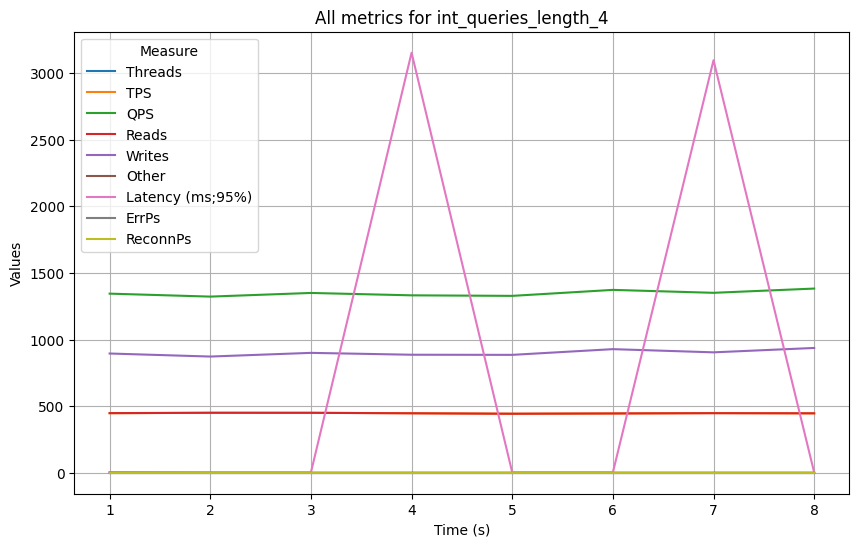
\includegraphics[width=\textwidth]{PNGs/Join_Type/int_queries_length_4}
        \caption{\texttt{int\_queries\_length\_4}}
        \label{join-typ-int_queries}
    \end{subfigure}
    \hfill
    \begin{subfigure}[t]{0.48\textwidth}
        \centering
        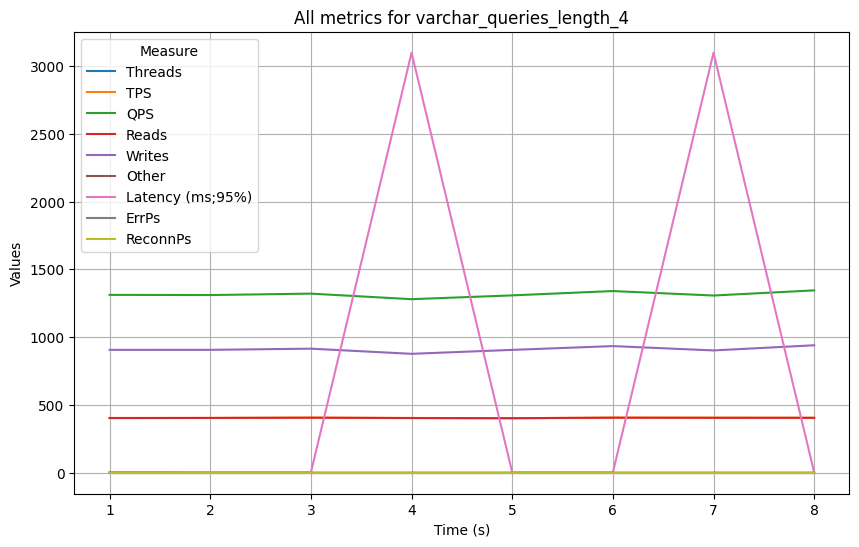
\includegraphics[width=\textwidth]{PNGs/Join_Type/varchar_queries_length_4}
        \caption{\texttt{varchar\_queries\_length\_4}}
        \label{join-typ-varchar_queries_length_4}
    \end{subfigure}
    \caption[Join-Typ: Skriptvergleich]{Die Grafik zeigt alle Metriken für die jeweiligen Skripte}
    \label{fig:join-typ-comp-script}
\end{figure}
\vspace{-20pt}

Wenn alle vier Skripte miteinander verglichen werden sollen, können die Abbildungen aus~\ref{fig:join-typ-comp-metric} herangezogen werden.
Was die Lesegeschwindigkeit angeht, kann man erkennen, dass \texttt{INT} eine etwa 10\% bessere Lese-Performance hat als \texttt{VARCHAR} bei einer Länge von 4.
Aus dem Vergleich von den unterschiedlichen Längen mit \texttt{INT} kann man schließen, dass er Einfluss nicht sonderlich groß ist.
In diesem Fall ist sogar die Variante mit 16 Stellen im Durchschnitt etwas schneller als die mit 4.
Bei \texttt{VARCHAR} ist deutlich erkennbar, dass die Abfrage umso langsamer wird, je länger die Zeichenkette ist.
Dennoch ist der Unterschied zwischen den Datentypen größer als innerhalb der verschiedenen Längen von \texttt{VARCHAR}.
Es ist auch zu erkennen, dass die Werte bis auf wenige Ausnahmen sehr konstant bleiben und es keine großen Schwankungen gibt.
Aus der Gesamtstatistik in~\ref{fig:join-typ-hex} kann ein ähnliches Verhalten abgeleitet werden.
Bei der Schreibgeschwindigkeit kann man kaum Unterschiede erkennen und auch bei der Latenz liegen alle Varianten nah aneinander.

\vspace{-5pt}
\begin{figure}[H]
    \centering
    \begin{subfigure}[t]{0.48\textwidth}
        \centering
        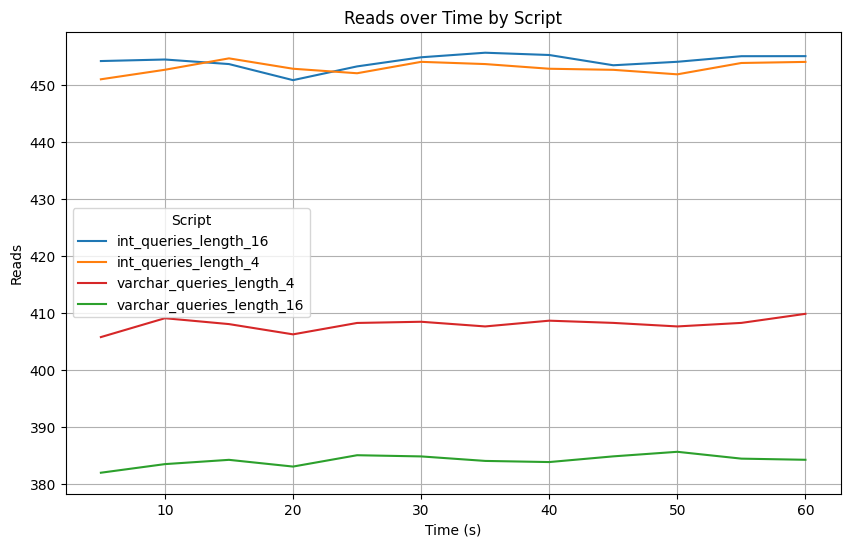
\includegraphics[width=\textwidth]{PNGs/Script/Join_Typ/join-type/Reads}
        \caption{Reads}
        \label{join-typ-reads}
    \end{subfigure}
    \hfill
    \begin{subfigure}[t]{0.42\textwidth}
        \centering
        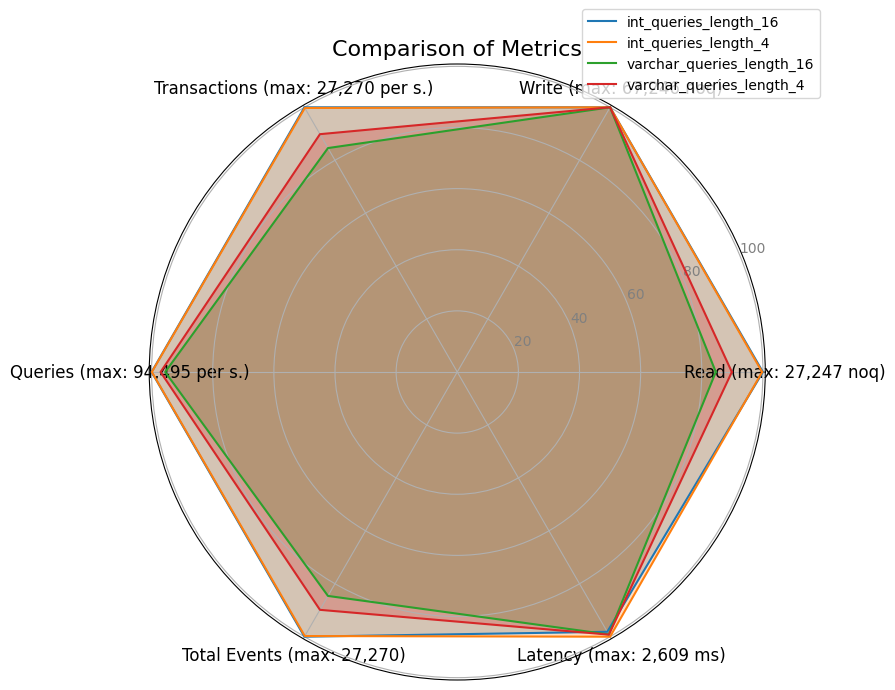
\includegraphics[width=\textwidth]{PNGs/Script/Join_Typ/join-type/statistics}
        \caption{Gesamtstatistik}
        \label{fig:join-typ-hex}
    \end{subfigure}
    \caption[Join-Typ: Metrikvergleich]{Die Grafik zeigt den Vergleich zwischen allen Skripten für die Metriken}
    \label{fig:join-typ-comp-metric}
\end{figure}
\vspace{-20pt}

\section{GitHub Actions}\label{sec:github-actions}

Im Verlauf der Bachelorarbeit kommen immer mehr Projekte mit unterschiedlichen Lua-Dateien, die alle das Orchestrator-Skript verwenden, dazu.
Manche dieser Projekte erfordern keine Anpassungen an dem Skript, während andere wiederum viele benötigen.
Das Problem dabei ist, dass man durch die Komplexität des Skripts schnell den Überblick über die Auswirkungen der Änderungen auf andere Projekte verliert.
Um sicherzugehen, müssen die Benchmarks für alle Projekte durchgeführt und anschließend die Output-Ergebnisse überprüft werden.
Dazu muss jedes Skript nacheinander ausführt werden, was zum einen zeitintensiv ist und zum anderen hohe Lasten für den lokalen Rechner bedeutet.
Das Vorgehen könnte man zeitlich optimieren, indem man die Skripte parallel ausführt, aber auch das würde nicht das Problem der hohen Lasten und des manuellen Aufwands lösen.
Eine deutlich bessere Variante ist das Automatisieren dieser Befehle unabhängig von dem lokalen Rechner auf virtuellen Maschinen in der Cloud.
Als Plattform für Continuous Integration und Continuous Delivery (CI/CD) wurde GitHub Actions gewählt (\cite{github_action_doku}).
Mit GitHub Actions kann man Workflows erstellen, die bei einem bestimmten Event getriggert werden und anschließend eine Anzahl von Aufträgen nacheinander oder gleichzeitig ausführen können.
Jeder Auftrag (engl.\ Job) wird innerhalb eines eigenen Runners der virtuellen Maschine in einem Container ausgeführt und kann über einen oder mehrere Schritte verfügen.
Die Schritte können wiederum beliebige Shell-Befehle, Skripte oder Aktionen ausführen.

Im vorherigen Kapitel wurde gezeigt, wie das Hauptskript für das Beispiel auf dem lokalen Rechner ausgeführt werden kann (\ref{lst:tools-orchestrator-command}).
Jetzt werden diese Informationen für alle Projekte gebraucht, die getestet werden sollen.
Es werden immer die Pfade zu den Lua-Skripten benötigt, die getestet werden sollen, sowie in einigen Fällen die zusätzlich definierten Variablen.
Diese Pfade und Variablen werden in einer JSON-Datei gesammelt und jedem Projekt wird ein Name zugewiesen, hier z.B.\ \texttt{join-type}.

\vspace{-8pt}
\lstinputlisting[
    language=Json,
    caption=JSON-Datei mit dem Join-Typ Beispiel,
    label={lst:tools-script-configuration},
    style=custom_daniel,
    basicstyle=\ttfamily\scriptsize,
]{Scripts/Grundlagen/10_Pattern.json}
\vspace{-5pt}

Damit das Hauptskript ausgeführt werden kann, müssen im ersten Job die Daten dieser JSON-Datei verarbeitet und bestimmte Variablen, wie beispielsweise der Output-Ordner, definiert werden.
Zudem müssen alle Namen der verschiedenen Projekte in einer Liste zusammengefügt und als Output für den nächsten Job bereitgestellt werden.
Der nächste Auftrag ist verantwortlich für das eigentliche Durchführen der Benchmarks und wird erst gestartet, wenn der Vorherige beendet ist.
Um die Vorteile des gleichzeitigen Ausführens der Aufträge zu nutzen, muss die Matrixstrategie verwendet werden.
Bei der Matrixstrategie kann man eine Liste von Variablen angeben, um mehrere Auftragsausführungen parallel zu erstellen.
In diesem Fall wird dafür die Liste mit den unterschiedlichen Projektnamen genutzt.

Damit die einzelnen Benchmarks ausgeführt werden können, müssen innerhalb der Matrixausführung einige Vorbereitungen getroffen werden.
Zuallererst müssen, abhängig vom Projektnamen, die entsprechenden Variablen aus der JSON-Datei, die im ersten Job erstellt wurden, geladen und exportiert werden.
Anschließend werden die Dependencies für Sysbench und die Python-Libraries installiert sowie die Datenbank-Container mit passenden Konfigurationen gestartet und vorbereitet.
Nach diesen Schritten kann das Hauptskript ausgeführt werden und die Outputdateien werden am angegebenen Pfad erstellt.

Um Zugriff auf diese Dateien zu erhalten, müssen sie als GitHub Artifact hochgeladen werden.
Die GitHub Artifacts können anschließend entweder über die GitHub REST API oder die Übersicht des Workflows auf der GitHub-Webseite als Zip-Datei heruntergeladen werden.
Als letzten Schritt, nach Beendigung beider vorangegangenen Jobs, können alle GitHub Artifacts des aktuellen Workflows heruntergeladen und gemeinsam als ein neues Artifact wieder hochgeladen werden.
Dadurch entfällt beispielsweise bei 10 Projekten die Notwendigkeit, 10 Zip-Dateien einzeln herunterzuladen und zu entpacken, um die Änderungen in den Dateien zu überprüfen.
Wenn fehlerhafte Änderungen den Workflow triggern, kann es dazu kommen, dass je nach Fehler unterschiedliche Jobs oder Steps nicht erfolgreich ausgeführt werden und damit der komplette Workflow scheitert.

Der Workflow wird in einer YAML-Datei im Ordner ~\texttt{.github/workflows/} definiert.
Zunächst muss man den Namen des Workflows festlegen und anschließend, wann er getriggert werden soll.
Dies kann beispielsweise manuell auf GitHub mit dem Tag \texttt{workflow\_dispatch} oder bei jedem Push mit \texttt{push} geschehen.
Zudem kann der Trigger auch auf bestimmte Dateien oder Ordner beschränkt werden.
Als Nächstes kann man unter dem Tag \texttt{jobs} die verschiedenen Aufträge definieren.
Der Schlüssel \texttt{outputs} beschreibt die Ausgaben eines Jobs, die von anderen Jobs verwendet werden können, während \texttt{steps} die Aufgaben festlegt, die innerhalb eines Jobs ausgeführt werden.
Unter dem Tag \texttt{env} muss man die Umgebungsvariablen definieren, dazu gehören zum Beispiel beim zweiten Job die Länge der Durchführung des Benchmarks.
Wenn es sich um vertrauliche Informationen handelt, sollte man GitHub Secrets verwenden.
Ein Beispiel dafür wäre das Downloaden der Artefakte im letzten Job, um einen gemeinsamen Output-Ordner zu erstellen.
Dafür wird die GitHub REST API benötigt, die ein vertrauliches \texttt{Personal Access Token} erfordert, welches Repository- sowie Lese- und Schreibrechte für GitHub Registries besitzt.
Die Workflow-Datei für das Durchführen der Benchmarks sieht in verkürzter Form wie folgt aus:

\vspace{-5pt}
\lstinputlisting[
    language=yaml,
    caption=Ausschnitt aus der Workflow-Datei,
    label={lst:tools-workflow-yaml},
    style=custom_daniel,
    basicstyle=\ttfamily\scriptsize,
]{Scripts/Grundlagen/11_Workflow.yaml}
\vspace{-5pt}

\section{Optimierung des Workflows}\label{sec:optimierung-des-workflows}

Es gibt verschiedene Möglichkeiten, die Laufzeit und den Ressourcenverbrauch des Workflows zu optimieren.
Zum einen kann man die zu installierenden Abhängigkeiten mithilfe von GitHub Caches (\cite{github_cache_doku}) speichern.
Dies bietet sich besonders deswegen an, da sich die Abhängigkeiten über die Workflows hinweg nur selten ändern.
Falls sich doch etwas ändert, kann man beispielsweise die \texttt{requirements.txt}-Datei anpassen.
Dadurch werden einmalig alle Abhängigkeiten neu installiert und anschließend im Cache abgelegt.
Falls sich bis zum nächsten Workflow keine Änderungen an den Abhängigkeiten ergeben, wird der Cache automatisch heruntergeladen.
Der Zeitgewinn in diesem Beispiel ist jedoch nur gering und beträgt nur wenige Sekunden pro Workflow.

%\vspace{-5pt}
%\lstinputlisting[
%    language=yaml,
%    caption=Speichern der Abhängigkeiten im Cache,
%    label={lst:tools-cache-yaml},
%    style=custom_daniel,
%]{Scripts/Grundlagen/12_Cache.yaml}
%\vspace{-5pt}

Deutlich mehr Zeit und Ressourcen kann man aber sparen, wenn man zwischen zwei unterschiedlichen Arten von Dateien unterscheidet.
Denn zum einen gibt es Dateien, die die Ergebnisse von allen Skripten beeinflussen.
Dazu gehören das Workflow-Skript und die JSON-Datei, aber auch das Orchestrator-Skript und die darin verwendeten Python-Skripte.
Die Ordner, die in der JSON angegeben werden, die beeinflussen aber nur sich selbst und nicht die anderen Skripte.
Beispielsweise, wenn in Projekt A die Anzahl an Zeilen geändert wird, die in eine Tabelle eingefügt werden, hat dies keinen Einfluss auf das Ergebnis von Projekt B oder C\@.
Daher würde es sich anbieten, die Benchmarks für Projekt A neu durchzuführen, während für Projekte B und C jeweils der letzte erfolgreiche Output-Ordner verwendet werden könnte.
Als Endresultat könnte damit die neue Durchführung von Projekt A zusammen mit der alten Ausführung der Projekte B und C in einer Zip-Datei hochgeladen werden.
Dadurch wird nur ein Drittel der eigentlichen Ressourcen verbraucht, wenn man davon ausgehen würde, dass alle 3 Projekte gleich viel Zeit benötigen würden.

Für die Implementierung dieser Optimierung müssen zunächst die allgemeinen Skripte sowie die benötigten Ordner mit den Lua-Skripten, die für das jeweilige Skript in der JSON-Datei erforderlich sind, gehasht werden.
Diese beiden Hashes können zusammen mit den Testtypen kombiniert werden.
Damit ergibt sich die folgende Struktur für den Namen:

\vspace{-5pt}
\begin{lstlisting}[language=yaml,label={lst:tools-hash_name},style=custom_daniel]
NAME="${{ matrix.test-type }}-${{ env.hash }}-${{ env.general_hash }}"
\end{lstlisting}
\vspace{-5pt}

Nachdem die JSON im ersten Job geladen wurde, wird nicht direkt mit dem zweiten und der damit verbundenen Installation der Abhängigkeiten fortgefahren.
Stattdessen werden zunächst die unterschiedlichen Pfade gehasht und der entsprechende Name erstellt.
Falls kein Ordner mit diesem Namen existiert, wird wie bisher fortgefahren.
Existiert jedoch bereits ein Ordner mit diesem Namen, werden alle weiteren Schritte nach dem Extrahieren der Werte aus der JSON im Job \texttt{run-tests} übersprungen.
Dadurch erspart man sich die Installation der Abhängigkeiten, das Starten der Datenbank-Container sowie das Ausführen des Orchestrator-Skripts.

Als letztes stellt sich die Frage, wo die Ordner mit den berechneten Namen gespeichert und beim nächsten Run wieder heruntergeladen werden sollen.
Zum einen kann man Lösungen in GitHub selbst verwenden.
Zum einen würde sich wieder eine GitHub Cache-Lösung anbieten, aber tatsächlich sind GitHub Artifacts für das Sichern von Dateien besser geeignet (\cite{github_cache_doku}).
Eine andere mögliche Lösung wäre die Nutzung expliziter Branches ausschließlich für die Sicherung der Dateien, bei der die GitHub Action über Schreibberechtigungen verfügen muss.
Das Problem ist dabei, dass durch Timing-Probleme beim Pushen ein paralleler Workflow den Code zwischen Rebase, Commit und Push verändert haben könnte, wodurch nach einem verhinderten Push erneut ein Rebase nötig wird.
Die Implementierung dieser Variante hat dieses Problem bestätigt.
Des Weiteren eignen sich auch Cloud-Speicherlösungen sehr gut, um die Ordner zu speichern und wieder herunterzuladen.
Dazu gehören von Google Cloud Storage (GCS), AWS S3 oder MS Azure Storage, die sich zusammen mit GitHub Artifacts am besten eignen.
Wie in der \texttt{workflow.yaml} zu erkennen ist, wurde die Lösung mit GitHub Artifacts gewählt.
Wenn man eine andere Lösung umsetzen möchte, dann muss man aber nur wenige Zielen im Workflow anpassen.